% ============================================================
\section{Distributed Linear Algebra Kernels and Krylov Solvers}
% ============================================================

\subsection{Overview and Motivation}

Large-scale numerical methods quickly become limited by more than
floating-point computation alone. Once the data and computational work
are distributed across multiple processes, communication and data
movement become part of the algorithm itself. The purpose of this
section is to build that distributed numerical foundation explicitly
using C++ and MPI.

The development follows the progression

$$
\text{MPI communication}
\rightarrow
\text{collective operations}
\rightarrow
\text{distributed data structures}
$$

$$
\rightarrow
\text{distributed linear algebra}
\rightarrow
\text{Krylov iterative solvers}.
$$

We begin close to the MPI layer, where the behavior of point-to-point
communication, synchronization, message ordering, and collective
operations can be studied directly. These ideas are then used to build
distributed vector and matrix operations rather than treating MPI as a
separate communication exercise.

The eventual goal of this section is a distributed implementation of
the Conjugate Gradient method. This provides a useful endpoint because
a single CG iteration brings together several of the components
developed along the way: distributed matrix--vector multiplication,
vector updates, inner products, and global reductions. It also provides
a natural foundation for the larger optimization systems developed in
later sections.


% ============================================================
\subsection{Point-to-Point Communication}
% ============================================================

MPI processes execute in separate address spaces, so a process cannot
directly access data owned by another process. Data dependencies across
processes therefore have to be expressed through explicit communication.
We started with point-to-point message passing to understand this model
before using higher-level collective operations.

The first implementation used \texttt{MPI\_Send} and
\texttt{MPI\_Recv} to exchange an integer between two ranks. Rank 0
sent the value to rank 1, rank 1 modified it, and the result was sent
back. This simple exchange was useful for identifying the pieces that
define an MPI message: the buffer, message size, datatype, source or
destination rank, tag, and communicator.

% ------------------------------------------------------------
\subsubsection{Blocking Communication and Deadlock}
% ------------------------------------------------------------

We next tested a deliberately unsafe communication pattern in which
both ranks attempted to send before receiving:

$$
P_0:\quad
\texttt{Send}(P_1)
\rightarrow
\texttt{Recv}(P_1),
$$

$$
P_1:\quad
\texttt{Send}(P_0)
\rightarrow
\texttt{Recv}(P_0).
$$

With a small integer message, the program completed normally. This was
initially misleading: the communication pattern appeared valid because
the MPI implementation could buffer the small outgoing messages.

The same experiment was then repeated with large buffers. In this case,
both ranks stalled in their send operations because neither had reached
the corresponding receive. The experiment exposed the circular
dependency that was hidden by buffering in the small-message case.

A safe blocking version was obtained by reversing the order on one
rank:

$$
P_0:\quad
\texttt{Send}
\rightarrow
\texttt{Recv},
\qquad
P_1:\quad
\texttt{Recv}
\rightarrow
\texttt{Send}.
$$

The main lesson was that a communication pattern should not depend on
MPI's internal buffering for correctness. Code that works for a small
message can deadlock when the message size or communication protocol
changes.

% ------------------------------------------------------------
\subsubsection{Nonblocking Communication}
% ------------------------------------------------------------

We then replaced the blocking exchange with
\texttt{MPI\_Irecv} and \texttt{MPI\_Isend}. Each process first posted
its receive, initiated its send, and then waited for both operations to
complete:

$$
\texttt{Irecv}
\rightarrow
\texttt{Isend}
\rightarrow
\texttt{Waitall}.
$$

Unlike a blocking call, an immediate MPI operation initiates the
communication without requiring it to be complete when the function
returns. The associated buffers therefore remain part of an outstanding
communication request until completion is established. In particular,
a send buffer should not be modified before the send completes, and a
receive buffer should not be used before the receive completes.

This structure also creates the possibility of overlapping useful work
with communication:

$$
\texttt{Irecv}
\rightarrow
\texttt{Isend}
\rightarrow
\text{independent computation}
\rightarrow
\texttt{Waitall}.
$$

Nonblocking communication is not automatically faster. If
\texttt{MPI\_Waitall} immediately follows the communication calls,
there may be little computation available to hide the communication
cost. The importance here is that the communication and computation
phases no longer have to be strictly sequential.

% ------------------------------------------------------------
\subsubsection{Chain and Ring Communication}
% ------------------------------------------------------------

After the two-process experiments, the communication pattern was
extended across multiple ranks.

The first topology was a chain. Rank 0 initialized a token and sent it
to rank 1. Each subsequent rank received the token from its predecessor,
incremented it, and forwarded it to the next process:

$$
P_0
\rightarrow
P_1
\rightarrow
P_2
\rightarrow
\cdots
\rightarrow
P_{P-1}.
$$

Starting from zero, the final rank should receive

$$
P-1.
$$

The implementation was tested with $P=2$, $4$, and $8$, producing final
values $1$, $3$, and $7$, respectively.

The chain was then closed into a ring. For rank $r$, its neighboring
processes were defined as

$$
\operatorname{prev}(r)
=
(r-1+P)\bmod P,
$$

$$
\operatorname{next}(r)
=
(r+1)\bmod P.
$$

Rank 0 initiated the token. Every other rank received from its previous
neighbor, incremented the token, and forwarded it to its next neighbor.
The last rank therefore returned the token to rank 0.

Although the ring has no physical endpoints, rank 0 serves as the
algorithmic initiator in this experiment. The blocking implementation
remains safe because rank 0 begins with a send while the remaining ranks
begin with receives, providing an initial matching communication pair
rather than creating a circular wait.

These experiments established the communication patterns used in the
next stage. In particular, the ring topology provides a direct path
from point-to-point communication to implementing collective operations
explicitly.



% ============================================================
\subsection{Collective Communication}
% ============================================================

Collective operations involve all processes in a communicator and form
an important part of distributed numerical algorithms. Rather than
treating these operations as black boxes, we first implemented one
collective explicitly using point-to-point communication.

The first operation considered was Allgather. Each rank begins with a
local chunk of $N$ values. After the operation, every rank should hold
the chunks contributed by all $P$ processes. Thus, the final buffer on
each rank contains $PN$ values.

% ------------------------------------------------------------
\subsubsection{Ring-Based Allgather}
% ------------------------------------------------------------

A ring communication pattern was used to construct the Allgather
operation. For rank $r$, the neighboring processes are

$$
\operatorname{prev}(r)=(r-1+P)\bmod P,
$$

$$
\operatorname{next}(r)=(r+1)\bmod P.
$$

Initially, every rank places its own chunk in the appropriate location
of its output buffer. Communication then proceeds for $P-1$ rounds.
During each round, every rank simultaneously sends one chunk to its
next neighbor and receives one chunk from its previous neighbor.

For example, with four ranks containing the values $10$, $20$, $30$,
and $40$, the first communication round is

$$
P_0 \rightarrow P_1:10,
\qquad
P_1 \rightarrow P_2:20,
$$

$$
P_2 \rightarrow P_3:30,
\qquad
P_3 \rightarrow P_0:40.
$$

In the next round, each process forwards the chunk that it received in
the previous round. Since every rank begins with one chunk and learns
one new chunk per round, exactly $P-1$ rounds are required before every
rank has all $P$ chunks.

An important implementation detail is the distinction between the
process that sends a message and the process that originally owned the
data. After the first round, these are generally different. At
communication step $s$, the original owner of the chunk received by
rank $r$ is

$$
\operatorname{owner}(r,s)
=
(r-s-1+P)\bmod P.
$$

This index determines where the received chunk belongs in the final
gathered buffer.

The communication in each round was implemented using
\texttt{MPI\_Irecv}, \texttt{MPI\_Isend}, and
\texttt{MPI\_Waitall}. All ranks therefore participate in every
communication round rather than gathering the data sequentially at a
single process.

% ------------------------------------------------------------
\subsubsection{Correctness Verification}
% ------------------------------------------------------------

The custom implementation was checked directly against
\texttt{MPI\_Allgather}. Each rank executed both versions and compared
the resulting buffers locally. The local correctness indicators were
then combined using

$$
\texttt{MPI\_Reduce}
+
\texttt{MPI\_LAND},
$$

so that the test passed only when the custom and native results agreed
on every rank.

The implementation was tested for multiple process counts and chunk
sizes. All configurations used in the benchmark study passed the
correctness check.

% ------------------------------------------------------------
\subsubsection{Benchmark Methodology}
% ------------------------------------------------------------

Timing a distributed operation requires accounting for the fact that
different ranks may finish at slightly different times. Before each
measurement, the processes were synchronized using
\texttt{MPI\_Barrier}. Each rank then measured its local execution time
using \texttt{MPI\_Wtime}.

For repetition $i$, if $T_i^{(r)}$ denotes the time measured by rank
$r$, the runtime of the distributed operation was taken to be

$$
T_i
=
\max_{0\leq r<P} T_i^{(r)}.
$$

The maximum was computed using \texttt{MPI\_Reduce} with
\texttt{MPI\_MAX}. This reflects the fact that the collective operation
is not effectively complete until its slowest participating rank has
finished.

To reduce first-use effects, each implementation was executed for 10
warmup iterations before measurement. The benchmark then used 100
measured repetitions. Minimum, median, mean, and maximum runtimes were
recorded, with the median used as the main comparison statistic.

% ------------------------------------------------------------
\subsubsection{Scaling Results}
% ------------------------------------------------------------

The experiment varied both the number of MPI processes $P$ and the
number of integers contributed by each process $N$. The median runtimes
are shown below.

\begin{table}[ht]
	\centering
	\begin{tabular}{rrrrr}
		\toprule
		$P$ & $N$ & Ring (ms) & MPI (ms) & Ring/MPI \\
		\midrule
		2 & $10^4$ & 0.147 & 0.00330 & 44.7 \\
		2 & $10^5$ & 1.447 & 0.0474  & 30.6 \\
		2 & $10^6$ & 15.454 & 0.683  & 22.6 \\
		\midrule
		4 & $10^4$ & 0.346 & 0.0250 & 13.8 \\
		4 & $10^5$ & 2.946 & 0.152  & 19.3 \\
		4 & $10^6$ & 32.097 & 3.705  & 8.66 \\
		\midrule
		8 & $10^4$ & 1.114 & 0.0703 & 15.9 \\
		8 & $10^5$ & 10.800 & 0.652 & 16.6 \\
		8 & $10^6$ & 111.026 & 13.539 & 8.20 \\
		\bottomrule
	\end{tabular}
	\caption{Median runtime of the custom ring Allgather and
		\texttt{MPI\_Allgather} over 100 measured repetitions.}
	\label{tab:ring-allgather}
\end{table}

% ------------------------------------------------------------
\subsubsection{Performance Interpretation}
% ------------------------------------------------------------

Two scaling effects are visible in Table~\ref{tab:ring-allgather}.
First, runtime increases approximately linearly with chunk size once
the messages become sufficiently large. For example, with $P=8$, the
ring implementation required approximately $1.11$ ms, $10.80$ ms, and
$111.03$ ms for chunk sizes $10^4$, $10^5$, and $10^6$, respectively.
This is consistent with the standard communication model

$$
T_{\mathrm{comm}}(m)
\approx
\alpha+\beta m,
$$

where $\alpha$ represents message latency and $\beta m$ represents the
cost associated with transferring $m$ units of data.

Second, increasing the number of processes increases the number of
communication rounds. The ring requires

$$
P-1
$$

rounds, and each process communicates one chunk during every round.
The amount of data sent by each process is therefore proportional to

$$
(P-1)N.
$$

The custom implementation is substantially slower than
\texttt{MPI\_Allgather} across all tested configurations. Part of this
difference comes from the simplicity of the implementation. In every
round, the received chunk is copied into the gathered buffer and then
copied again into the outgoing buffer for the next round. The native
MPI implementation can use optimized collective algorithms and
lower-level communication paths that are not reproduced here.

The purpose of the custom implementation is therefore not to outperform
the MPI library. Its value is that the communication rounds, data
ownership, synchronization, and scaling costs are explicit. These
details become important when collective communication is later used
inside distributed numerical kernels.


% ------------------------------------------------------------
% Future subsections
% ------------------------------------------------------------

%\subsection{Distributed Data Structures}
%
%\subsection{Distributed Vector Kernels}

%\subsection{Distributed Matrix--Vector Multiplication}

% ============================================================
\subsection{Distributed Matrix--Matrix Multiplication}
% ============================================================

We next consider dense matrix multiplication as a test case for distributed numerical computation. Unlike the communication exercises discussed earlier, this problem combines a substantial arithmetic workload with the need to distribute data and collect results. It therefore provides a useful setting for examining how MPI performance changes with both problem size and process count.

% ------------------------------------------------------------
\subsubsection{Problem Formulation}
% ------------------------------------------------------------

Given two dense matrices $A,B\in\mathbb{R}^{N\times N}$, our objective is to compute their product $C=AB$, where
\begin{equation}
	C_{ij}=\sum_{k=0}^{N-1}A_{ik}B_{kj}
\end{equation}

The conventional matrix multiplication algorithm requires $O(N^3)$ arithmetic operations. As $N$ increases, this cost grows rapidly, making the problem a natural candidate for parallel computation.

Our implementation uses double-precision floating-point arithmetic and stores matrices as contiguous, row-major arrays. We compare a serial implementation with an MPI implementation using a one-dimensional row decomposition. Both implementations use the same local multiplication kernel so that the comparison focuses on the effects of distributing the computation.

% ------------------------------------------------------------
\subsubsection{One-Dimensional Row Decomposition}
% ------------------------------------------------------------

We distribute the rows of matrix $A$ evenly among $P$ MPI processes. Each process is responsible for computing the corresponding rows of the output matrix $C$.

For simplicity, we restrict attention to configurations where $N$ is divisible by $P$. Each process therefore receives
\begin{equation}
	n_{\mathrm{local}}=\frac{N}{P}
\end{equation}
rows. Process $r$, indexed from zero, owns rows
\begin{equation}
	r\frac{N}{P},\ldots,(r+1)\frac{N}{P}-1
\end{equation}

An important feature of this decomposition is that every process requires access to the entire matrix $B$. We therefore distribute $A$ by rows but replicate $B$ across all processes.

This choice keeps the local computation straightforward. Once a process has its assigned rows of $A$ and a copy of $B$, it can calculate its portion of $C$ without communicating with other processes.

Since each process receives the same number of rows, the arithmetic workload is evenly divided. The computational complexity per process is approximately
\begin{equation}
	O\left(\frac{N^3}{P}\right)
\end{equation}

This is balanced in terms of operation count, although equal work does not necessarily imply equal execution time on a heterogeneous processor.

% ------------------------------------------------------------
\subsubsection{MPI Algorithm and Communication}
% ------------------------------------------------------------

The calculation begins on rank 0, which generates the input matrices using a fixed random seed. Matrix entries are sampled from a uniform distribution on $[-1,1]$, allowing the same inputs to be reproduced across experiments.

The MPI implementation proceeds through four main stages.

First, \texttt{MPI\_Scatter} distributes consecutive blocks of rows of $A$ to the processes. Next, \texttt{MPI\_Bcast} makes the complete matrix $B$ available to every process.

Each process then multiplies its local block of $A$ by $B$, producing its assigned rows of $C$. Finally, \texttt{MPI\_Gather} collects these rows on rank 0, reconstructing the complete result.

The local multiplication uses an $i$-$k$-$j$ loop ordering. For each entry of $A$, the algorithm updates a contiguous row segment of $C$ using a corresponding row of $B$. This improves memory-access locality compared with an implementation that repeatedly traverses columns of a row-major matrix.

All communication takes place outside the local multiplication kernel. This makes the implementation relatively simple to reason about: the processes exchange input data, perform independent computations, and then return their results.

The main trade-off is the replication of $B$. While it avoids communication during multiplication, every process must store an additional $N\times N$ matrix. The approach is therefore convenient for moderate problem sizes but is not necessarily the best choice for very large distributed systems.

% ------------------------------------------------------------
\subsubsection{Correctness Verification}
% ------------------------------------------------------------

Before examining performance, we verify that the distributed calculation agrees with the serial implementation.

Rank 0 computes a reference product using the serial multiplication kernel. After the MPI result has been gathered, we compare the two matrices using the maximum absolute error,
\begin{equation}
	e_{\max}
	=
	\max_{i,j}
	\left|
	C_{ij}^{\mathrm{MPI}}
	-
	C_{ij}^{\mathrm{serial}}
	\right|
\end{equation}

We accept a result when
\begin{equation}
	e_{\max}
	\leq
	10^{-10}
	\max\left(
	1,
	\max_{i,j}|C_{ij}^{\mathrm{serial}}|
	\right)
\end{equation}

All twelve required configurations passed this test. In every case, the reported maximum absolute error was zero. This is consistent with the serial and distributed implementations using the same arithmetic ordering for each output element.

These tests establish agreement with the serial reference for the matrices and configurations examined. They do not, by themselves, constitute a general proof of numerical correctness.

% ------------------------------------------------------------
\subsubsection{Benchmark Methodology}
% ------------------------------------------------------------

Experiments were performed on a Fedora Linux workstation equipped with an Intel Core i7-13620H processor, GCC 16.2.1, and Open MPI 5.0.9.

The processor has six performance cores and four efficiency cores, providing ten physical cores and sixteen logical CPUs. This distinction is important when interpreting the results for sixteen MPI processes, since these processes do not have sixteen independent physical cores available.

We tested four matrix sizes and three process counts:
\begin{equation}
	N\in\{2^6,2^8,2^{10},2^{12}\},
	\qquad
	P\in\{2^2,2^3,2^4\}
\end{equation}

This gives twelve configurations in total.

Execution times were measured using \texttt{MPI\_Wtime}. For each parallel repetition, the elapsed time was measured across the complete scatter, broadcast, computation, and gather sequence. The maximum elapsed time across MPI ranks was used as the parallel runtime, since the overall calculation cannot be considered complete until all processes have finished.

We performed several warm-up runs before collecting measurements and report the median execution time. The number of repetitions was reduced for larger matrices to keep the total benchmarking time manageable.

\begin{table}[htbp]
	\centering
	\caption{Benchmark repetition schedule.}
	\label{tab:matmul-repetitions}
	\begin{tabular}{ccc}
		\hline
		Matrix size $N$ & Warm-ups & Measured runs \\
		\hline
		64, 256 & 3 & 10 \\
		1024 & 2 & 5 \\
		4096 & 1 & 3 \\
		\hline
	\end{tabular}
\end{table}

During the initial experiments, we noticed that the serial reference time increased substantially in the sixteen-process configuration. Further inspection showed that Open MPI used different CPU-binding policies depending on the process count.

To make the speedup comparisons more consistent, we subsequently measured the serial reference independently, using a single MPI process bound to a physical core. These independent measurements are used throughout the analysis below.

% ------------------------------------------------------------
\subsubsection{Performance and Scalability Analysis}
% ------------------------------------------------------------

Table~\ref{tab:matmul-runtime} presents the median parallel execution times together with the independently measured serial baselines.

\begin{table}[htbp]
	\centering
	\caption{Median execution times in seconds.}
	\label{tab:matmul-runtime}
	\begin{tabular}{ccccc}
		\hline
		$N$ & Serial & $P=4$ & $P=8$ & $P=16$ \\
		\hline
		64   & 0.000577 & 0.000173 & 0.000143 & 0.000219 \\
		256  & 0.033969 & 0.008598 & 0.007210 & 0.004639 \\
		1024 & 2.182096 & 0.545535 & 0.461393 & 0.358664 \\
		4096 & 138.313363 & 36.982388 & 29.911572 & 23.350082 \\
		\hline
	\end{tabular}
\end{table}

\begin{figure}[htbp]
	\centering
	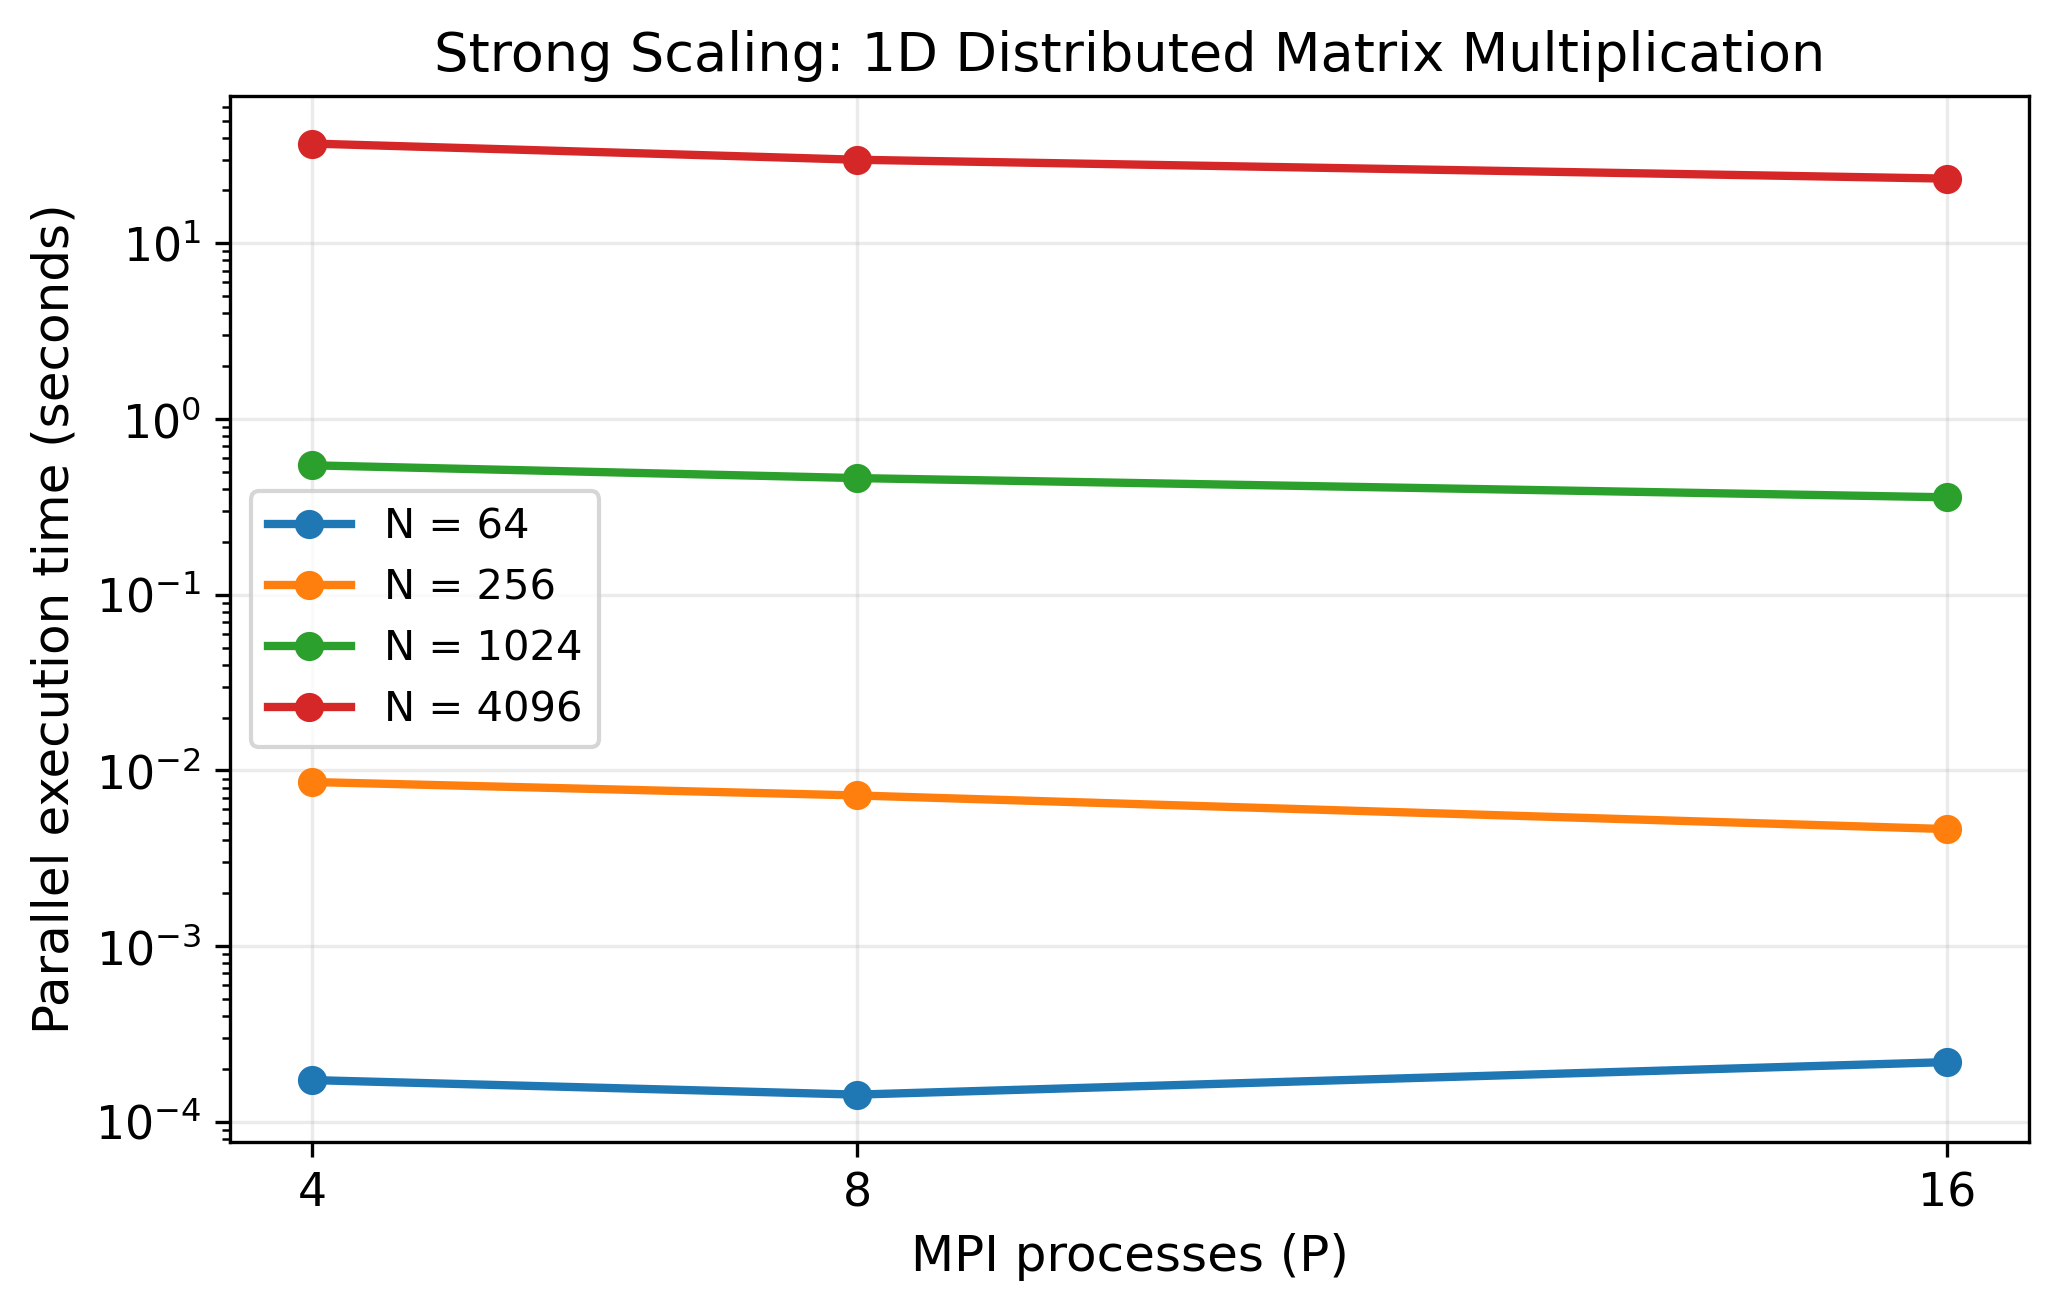
\includegraphics[width=0.85\textwidth]{../../results/figures/execution_time.png}
	\caption{Median parallel execution time as a function of MPI process count. The logarithmic vertical axis accommodates the large differences in runtime across matrix sizes.}
	\label{fig:matmul-runtime}
\end{figure}

The general trend is that distributing the computation reduces execution time. For $N=256$, $1024$, and $4096$, the fastest configuration uses sixteen processes. However, the improvement is considerably smaller than the fourfold reduction one might expect when increasing the process count from four to sixteen.

The smallest matrix behaves differently. For $N=64$, eight processes achieve the lowest execution time, while sixteen processes are slower than both four and eight. At this size, each process has relatively little arithmetic work, making communication, synchronization, and scheduling overhead more significant.

To quantify the benefits of parallel execution, we define speedup and parallel efficiency as
\begin{equation}
	S_P(N)=\frac{T_1(N)}{T_P(N)},
	\qquad
	E_P(N)=\frac{S_P(N)}{P},
\end{equation}
where $T_1(N)$ is the independently measured serial runtime and $T_P(N)$ is the parallel runtime using $P$ processes.

The resulting speedups are given in Table~\ref{tab:matmul-speedup}.

\begin{table}[htbp]
	\centering
	\caption{Measured speedup relative to the independent serial baseline.}
	\label{tab:matmul-speedup}
	\begin{tabular}{cccc}
		\hline
		$N$ & $P=4$ & $P=8$ & $P=16$ \\
		\hline
		64   & 3.335 & 4.035 & 2.635 \\
		256  & 3.951 & 4.711 & 7.322 \\
		1024 & 4.000 & 4.729 & 6.084 \\
		4096 & 3.740 & 4.624 & 5.923 \\
		\hline
	\end{tabular}
\end{table}

\begin{figure}[htbp]
	\centering
	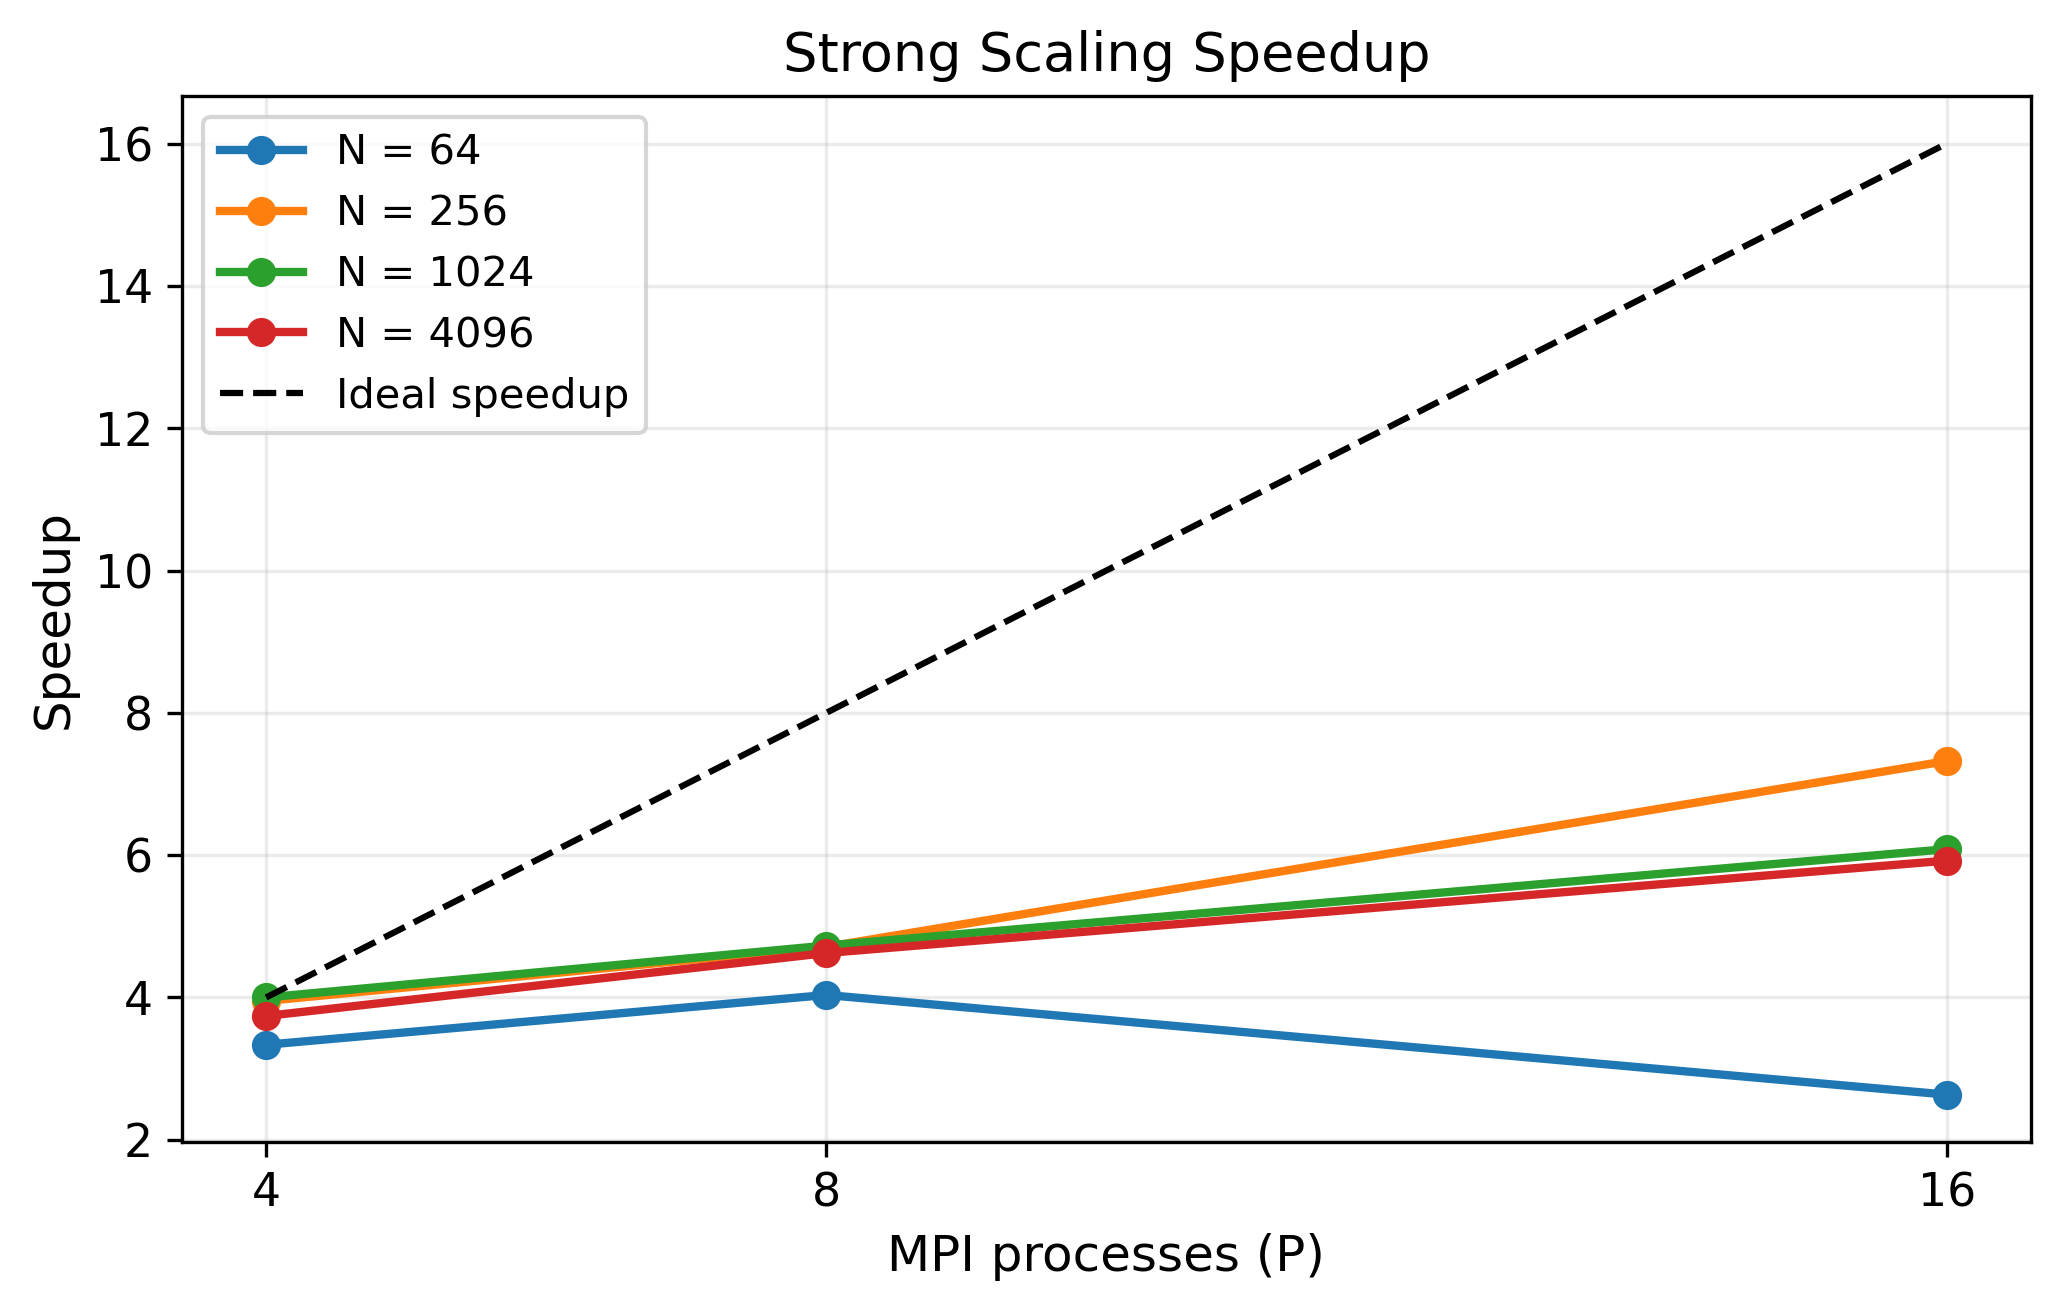
\includegraphics[width=0.85\textwidth]{../../results/figures/speedup.png}
	\caption{Measured speedup compared with ideal linear scaling, $S_P=P$. The measured curves increasingly depart from the ideal as the process count grows.}
	\label{fig:matmul-speedup}
\end{figure}

At four processes, the measured speedups are generally close to four. Increasing the number of processes to eight or sixteen continues to improve performance for the larger matrices, but the additional gains are smaller than ideal.

The corresponding parallel efficiencies are shown in Table~\ref{tab:matmul-efficiency}.

\begin{table}[htbp]
	\centering
	\caption{Parallel efficiency as a percentage.}
	\label{tab:matmul-efficiency}
	\begin{tabular}{cccc}
		\hline
		$N$ & $P=4$ & $P=8$ & $P=16$ \\
		\hline
		64   & 83.38 & 50.44 & 16.47 \\
		256  & 98.77 & 58.89 & 45.77 \\
		1024 & 100.00 & 59.12 & 38.02 \\
		4096 & 93.50 & 57.80 & 37.02 \\
		\hline
	\end{tabular}
\end{table}

\begin{figure}[htbp]
	\centering
	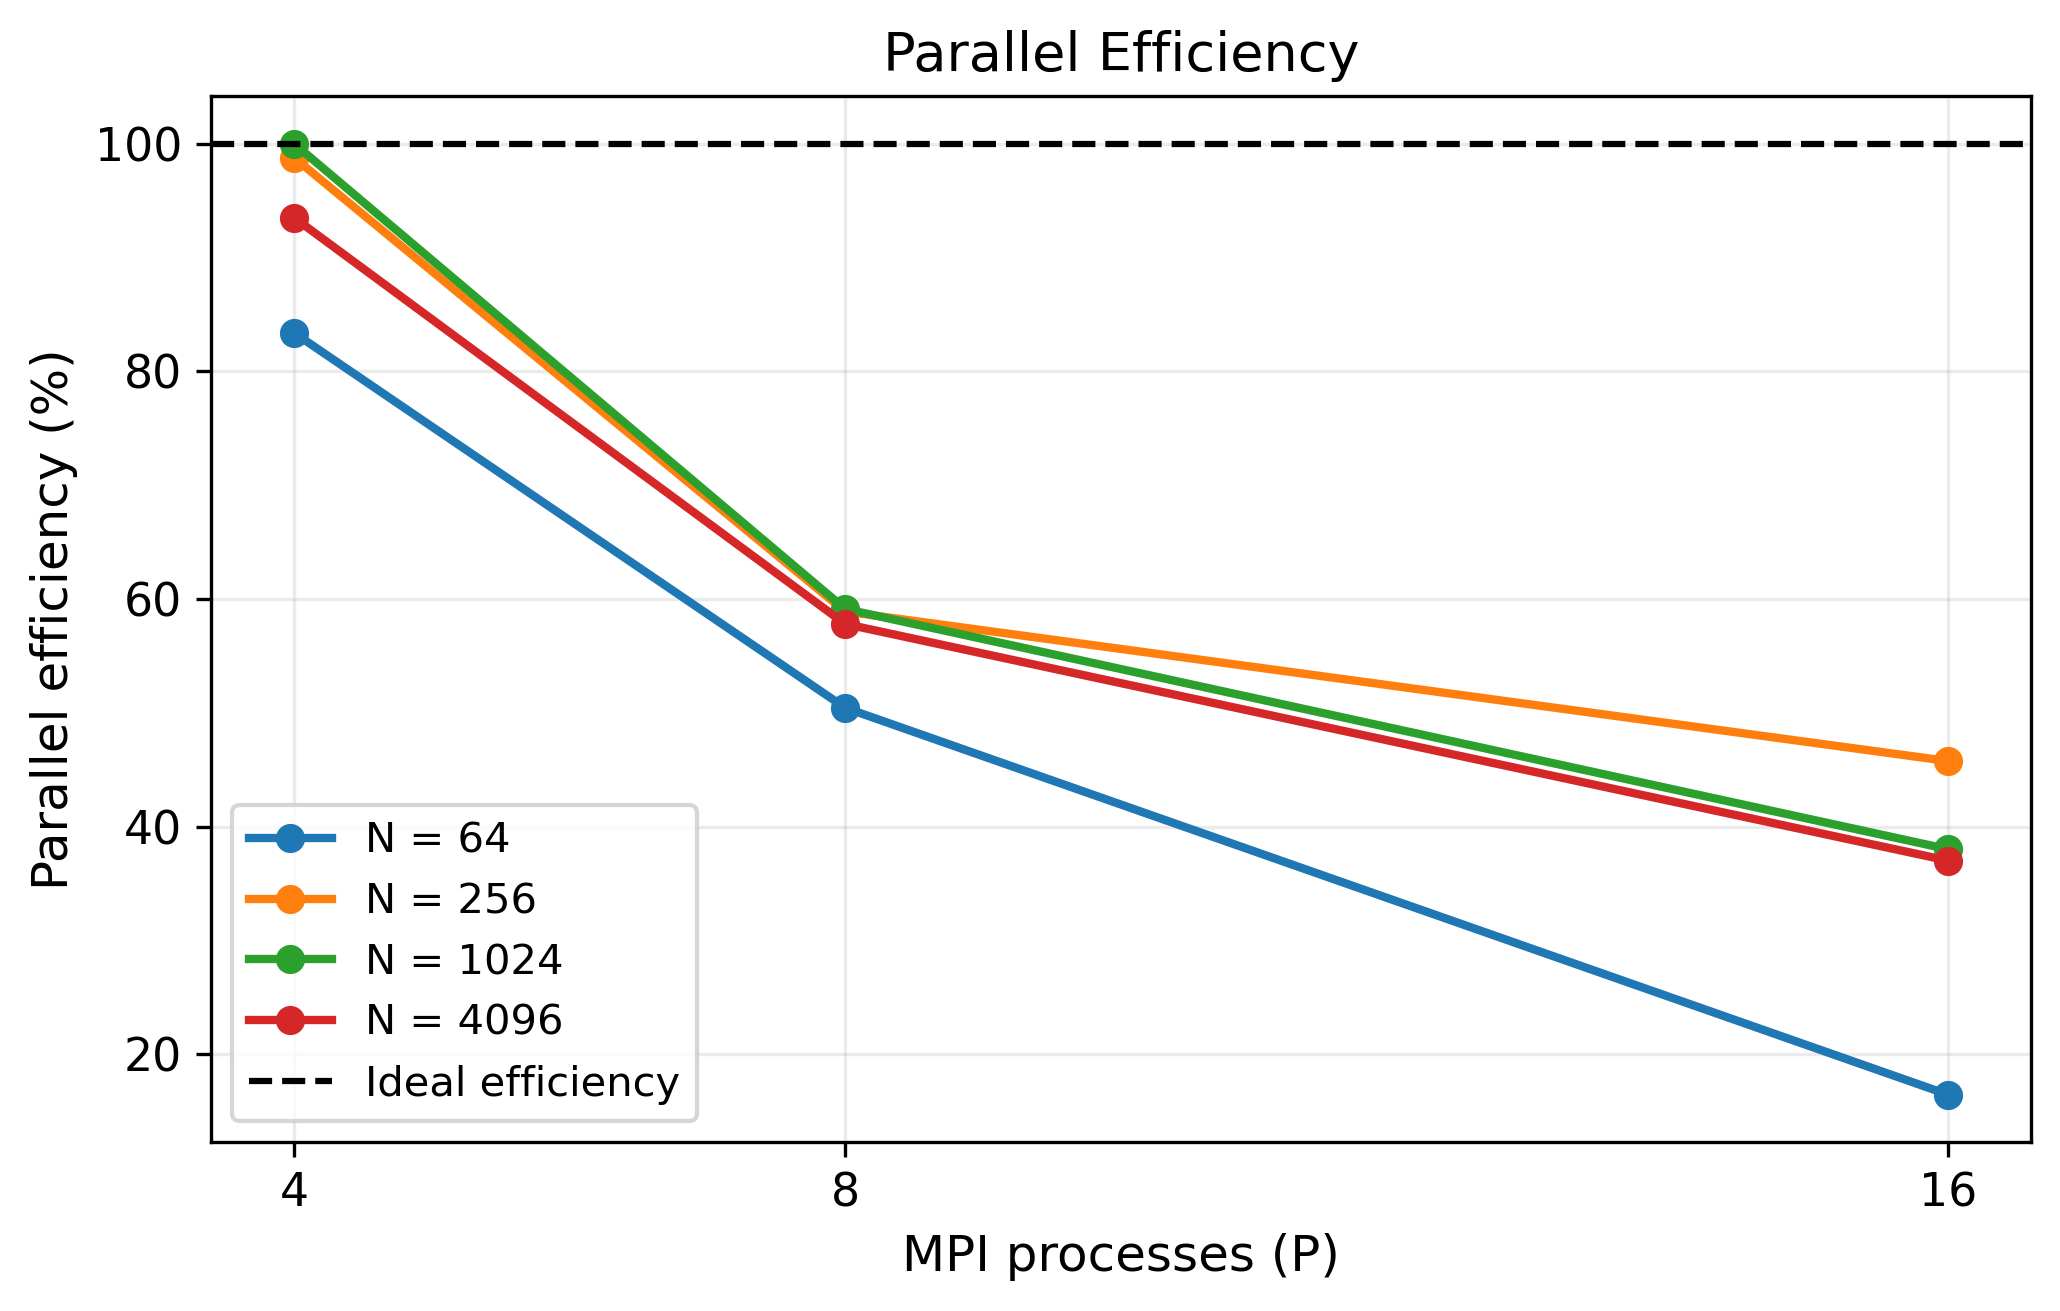
\includegraphics[width=0.85\textwidth]{../../results/figures/efficiency.png}
	\caption{Parallel efficiency for the four matrix sizes. Efficiency generally decreases as more MPI processes are introduced.}
	\label{fig:matmul-efficiency}
\end{figure}

The efficiency results make the limitations of the current implementation clearer. Although additional processes can reduce the total runtime, they do not provide proportional performance gains.

One reason is that communication does not disappear when the arithmetic workload is divided. Each process must receive its portion of $A$, obtain a copy of $B$, and participate in gathering the output.

To examine these costs, we also recorded timings for the scatter, broadcast, local computation, and gather phases. Figure~\ref{fig:matmul-phases} shows these measurements.

\begin{figure}[htbp]
	\centering
	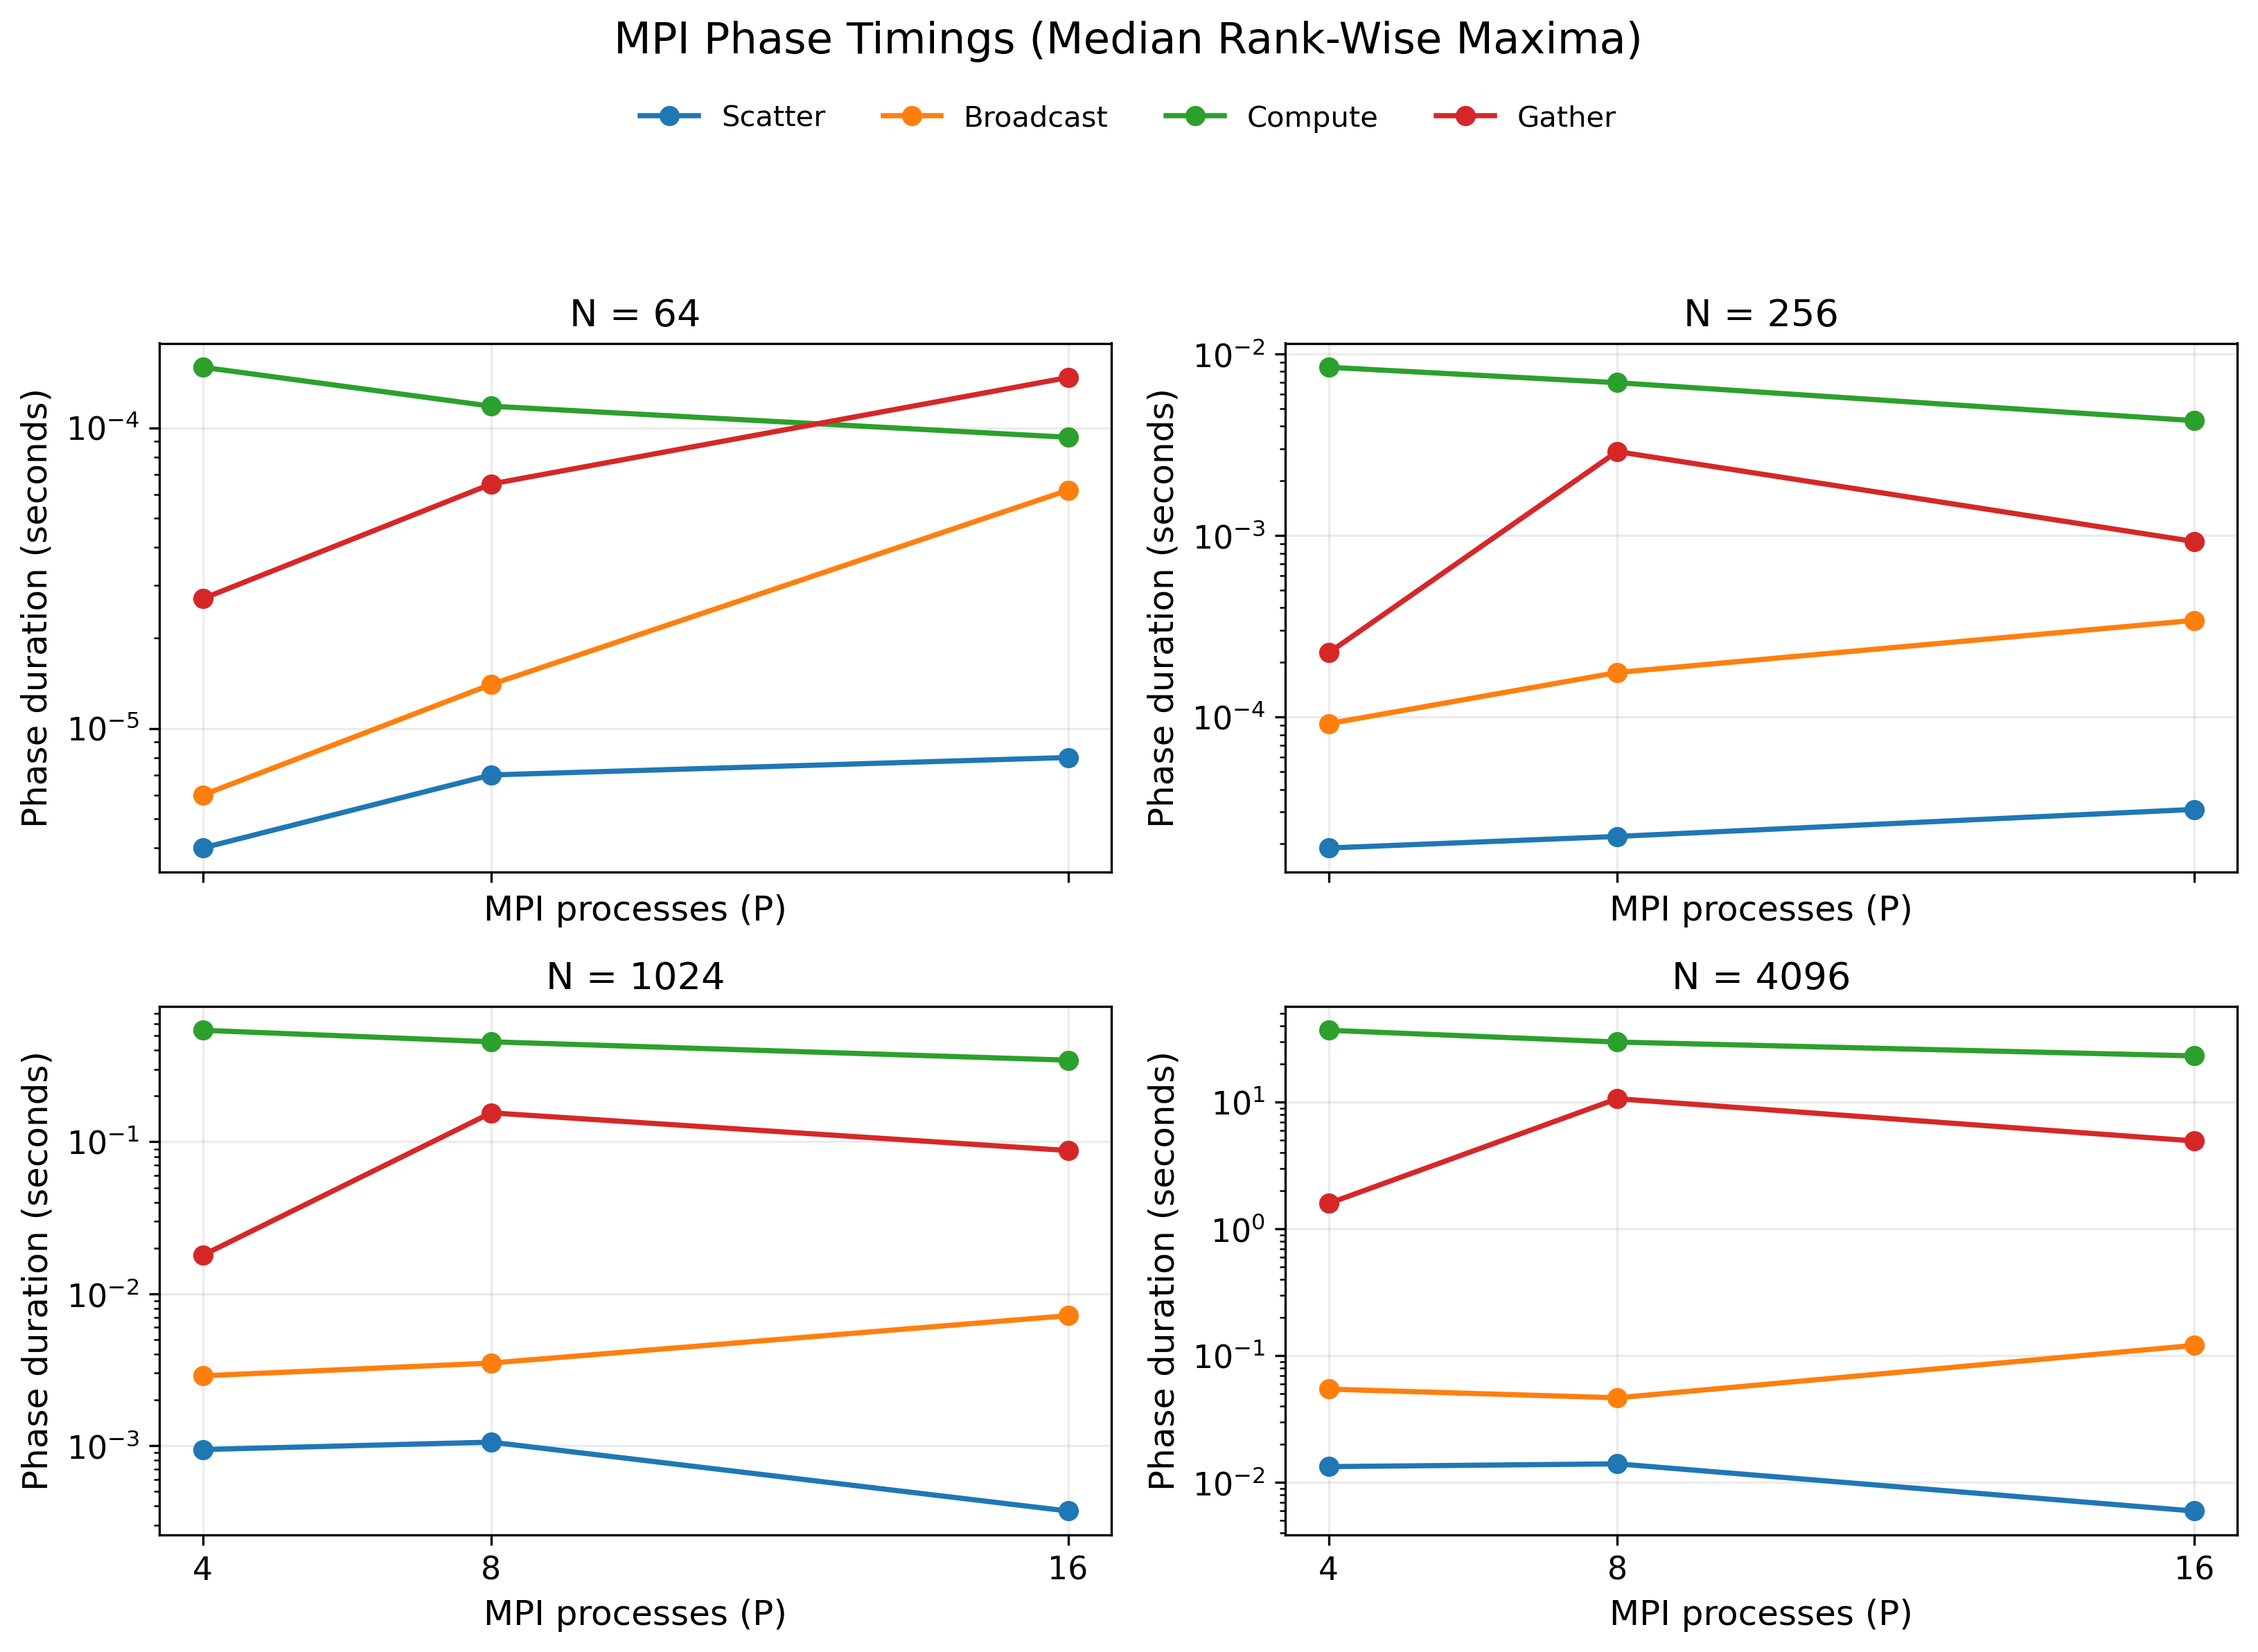
\includegraphics[width=0.95\textwidth]{../../results/figures/phase_timings.png}
	\caption{Median rank-wise maximum durations for the four execution phases. These independently summarized phase timings are not additive. In particular, collective timings may include waiting for other processes.}
	\label{fig:matmul-phases}
\end{figure}

For the larger matrices, local multiplication accounts for most of the measured execution time. Its duration decreases as the work is divided among more processes. Communication timings, however, do not follow the same trend.

The gather measurements are particularly variable. This does not necessarily mean that transferring the output matrix is expensive. A process entering \texttt{MPI\_Gather} early may spend time waiting for other processes to finish their local computations. Consequently, the measured collective duration can include synchronization delays as well as data movement.

Furthermore, the reported phase values are medians of rank-wise maxima computed separately for each phase. They should not be added together to reconstruct the total execution time.

The observed scaling can also be considered in the context of Amdahl's law. If a fraction $f$ of a computation cannot be parallelized, the idealized speedup using $P$ processors is
\begin{equation}
	S(P)=\frac{1}{f+\frac{1-f}{P}}
\end{equation}

This expression illustrates why even a relatively small non-parallelizable component can limit speedup as more processors are introduced.

Our measurements, however, include effects that are not captured by this simple model. Communication, synchronization, memory access, CPU scheduling, and contention between MPI processes all contribute to the observed runtime.

In particular, the sixteen-process experiments were performed on a processor with only ten physical cores. Some MPI ranks therefore share physical execution resources, and the machine also contains cores with different performance characteristics. We should not interpret these results as scaling measurements on sixteen identical, independent processors.

For these reasons, we use Amdahl's law to explain the general limitation on parallel speedup rather than attempting to infer an exact serial fraction from the measurements.

Overall, the experiments demonstrate that the one-dimensional decomposition provides substantial acceleration over serial matrix multiplication, but its scalability is limited by both the communication structure and the available hardware.

% ------------------------------------------------------------
\subsubsection{Limitations and Future Improvements}
% ------------------------------------------------------------

The implementation deliberately favors simplicity over maximum performance. Its most significant limitation is that every process stores the entire matrix $B$. As the matrix size and number of processes increase, this replication becomes increasingly expensive in terms of aggregate memory usage.

The current implementation also assumes that $N$ is divisible by $P$. Supporting arbitrary matrix sizes would require uneven row distributions, for example through \texttt{MPI\_Scatterv} and \texttt{MPI\_Gatherv}.

A natural next step is to investigate two-dimensional block decompositions, where both input matrices are distributed rather than replicating one of them everywhere. Blocked local multiplication and more careful communication scheduling may also improve performance.

Finally, testing on a larger computing cluster would help separate algorithmic scaling limitations from the effects of running many MPI processes on a single hybrid CPU.

Despite these limitations, the present implementation provides a working foundation for more advanced distributed linear algebra. It also illustrates an important practical lesson: parallel performance depends not only on how much arithmetic work is distributed, but also on how data is communicated and how the computation maps onto the underlying hardware.






%\subsection{Communication Algorithms and Topology}
%
%\subsection{Distributed Conjugate Gradient}
%
%\subsection{Performance and Scalability}